\documentclass[../main.tex]{subfiles}

\begin{document}
	\section{Kinematics}
		\begin{preamb}
			Kinematics is the study of the motion of objects. It can describe the way a thing moves in space over time. We will only cover one-dimensional motion in this chapter.
		\end{preamb}
	
		\subsection{Distance and Displacement}
		\pdef{Distance}{The distance traversed by an object in some time is the entire distance regardless of the direction of motion. The SI unit of distance is the metre [\si{\meter}].}
		Distances are a \textit{scalar} quantity.
		
		\pdef{Displacement}{The displacement of an object is the net change in position of an object. The SI unit of displacement is the meter [\si{\meter}].}
		Displacements are a \textit{vector} quantity. When reporting the displacement of an object, it is important to also state the \textbf{direction} from the origin point.
		
		\subsection{Average Speed, Average Velocity, and Instantaneous Velocity}
		\peqn{Average Speed}{The average speed of an object is given as}{\text{average speed} = \frac{\text{total distance}}{\text{total time}}}
		Soeed is a \textit{scalar} quantity.
		
		\pdef{Average Velocity}{The average velocity of an object is the change in rate of change of displacement of the object from the origin point.}
		
		\peqn{Average Velocity}{The average velocity of an object can be computed as}{\langle v \rangle = \frac{\Sigma s}{\Sigma t}}
		
		\pdef{Instantaneous Velocity}{The instantaneous velocity of an object is the rate of change of displacement of the object at some specific time. Mathematically, it is the derivative of the displacement function.}
		
		\peqn{Instantaneous Velocity}{The instantaneous velocity at a time \(t\) is computed as}{v(t) = \lim_{\Delta t \to 0} \frac{\Delta s}{\Delta t}}
		Velocity is a \textit{vector} quantity. When reporting the velocity of an object, it is important to also state the \textbf{direction} from the origin point.
		\subsection{Acceleration}
		\pdef{Acceleration}{Acceleration is the rate of change of velocity.}
		\peqn{Acceleration}{The acceleration of an object is computed as}{a = \frac{\Delta v}{\Delta t}}
		Acceleration is a \textit{vector} quantity. When reporting the acceleration of an object, the direction from the origin point must be stated.
		
		\subsection{Kinematic Graphs}
		A kinematic graph is a visual representation of the state of motion of the object over a period of time. A kinematic graph is useful in many situations, and should be drawn when you are stuck in a kinematics problem.
		
		\subsubsection{Displacement-time Graph}
		The displacement-time graph records the displacement of an object over a time period. The displacement is recorded on the vertical axis, the time is recorded on the horizontal axis.
		
		\begin{center}
			\begin{tikzpicture}
			\pgfplotsset{ticks=none}
			\begin{axis}[
				axis lines = left,
				xlabel = \(t\),
				ylabel = \(s\)
			]
				\addplot [domain=0:10] {x^3};
			\end{axis}
		\end{tikzpicture}
		\end{center}
		
		The gradient of a displacement-time graph tells us its \textbf{velocity}.
		
		\subsubsection{Velocity-time Graph}	
		The velocity-time graph records the velocity of an object over a time period. The velocity is recorded on the vertical axis, the time is recorded on the horizontal axis.
		
		\begin{center}
			\begin{tikzpicture}
			\pgfplotsset{ticks=none}
			\begin{axis}[
			axis lines = left,
			xlabel = \(t\),
			ylabel = \(v\)
			]
			\addplot [domain=0:10] {x^2};
			\end{axis}
			\end{tikzpicture}
		\end{center}
		
		The gradient of a velocity-time graph tells us its \textbf{acceleration}; the area under a velocity-time graph tells us the \textbf{displacement}.
		
		\subsection{Freefall}
		\pdef{Freefall}{An object is in freefall when the only force acting on it is due to gravity.}
		This means that the acceleration due to freefall is always equal to the local acceleration \(g\), and all other forces like air drag do not exist.
		\begin{center}
			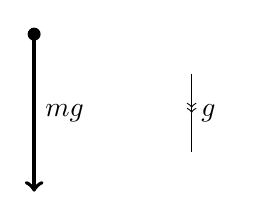
\begin{tikzpicture}
				\filldraw (0,0) circle (0.75mm);
				\draw [line width=0.5mm, ->] (0,0) -- (0,-2) node[pos=0.5, anchor=west] {\(mg\)};
				\draw [->>] (2,-0.5) -- (2,-1) node[anchor=west] {\(g\)};
				\draw (2,-1) -- (2,-1.5);
			\end{tikzpicture}
		\end{center}
		
		\subsection{Air drag}
		In real situations, air drag, or air resistance, is a resistive force that works against the weight of an object when falling. Air drag is proportional to the square of the velocity of an object.
		
		As an object falls, its velocity increases. Air drag then also increases. The acceleration of the object slowly decreases as the net force acting on the object is decreasing. 
		
		This continues until a point where the air drag is equal and opposite to the weight of the object. The object then experiences zero net force, and has zero acceleration, maintaining a constant velocity. 
		
		This constant velocity is \textbf{terminal velocity}.
		
\end{document}